
%\section{First Section}
%\subsection{WELCOME}


\subsection{Introduction}

\par Many image processing, computer graphics, and computer vision challenges can be described as "translating" an input image into a corresponding output image. A scene can be displayed as an RGB image, a gradient field, an edge map, a semantic label map, and so on, just as a thought can be expressed in English or French. We describe automatic image-to-image translation as the challenge of translating one possible representation of a scene into another, given adequate training data, in the same way that automatic language translation is defined. Despite the fact that the setting is always the same: forecast pixels from pixels, each of these jobs has traditionally been done with distinct, special-purpose gear. The purpose of this study is to create a common framework for all of these issues.

Many image processing, computer graphics, and computer vision challenges can be described as "translating" an input image into a corresponding output image. A scene can be displayed as an RGB image, a gradient field, an edge map, a semantic label map, and so on, just as a thought can be expressed in English or French. We describe automatic image-to-image translation as the challenge of translating one possible representation of a scene into another, given adequate training data, in the same way that automatic language translation is defined. Despite the fact that the setting is always the same: forecast pixels from pixels, each of these jobs has traditionally been done with distinct, special-purpose gear. The purpose of this study is to create a common framework for all of these issues.


GANs with conditions GANs aren't the first to be used in a conditional setting. GANs have been trained on discrete labels, text, and even images in previous and concurrent studies. Image prediction from a normal map, future frame prediction, product photo generation, and image generation from sparse annotations have all been solved by image-conditional models. Several other articles have employed GANs for image-to-image mappings, but they only used them unconditionally, relying on other terms (such as L2 regression) to condition the output on the input. Inpainting, future state prediction, image alteration directed by user constraints, style transfer, and superresolution are all topics covered in these publications. Each method was created with a specific application in mind. Nothing about our framework is application-specific.

Our generator and discriminator architectures are based on those used in Both the generator and the discriminator use convolution BatchNormReLu modules.
Several architectural choices for the generator and discriminator distinguish our method from previous work. Unlike previous work, we use a "U-Net"-based architecture for our generator, and a convolutional "PatchGAN" classifier for our discriminator, which only penalises structure at the scale of image patches. To capture local style statistics, a similar PatchGAN architecture was presented previously in. We show that this method works on a broader range of situations and study the impact of modifying the patch size.




\par  


\subsection{Satellite To Map Image Conversion}

\par  By using the GAN model, satellite photos can be converted to map images. Conditional adversarial networks are being investigated as a general-purpose solution to image-to-image translation difficulties. These networks not only learn the mapping from input to output image, but also the loss function that will be used to train the mapping. Image prediction from a normal map, future frame prediction, product photo generation, and image generation from sparse annotations have all been solved by image-conditional models. Several other articles have employed GANs for image-to-image mappings, but they only used them unconditionally, relying on other terms (such as L2 regression) to condition the output on the input. Not only do these networks learn the mapping from input to output image, but they also learn a loss function.


	\begin{figure}[h!]
    \centering
    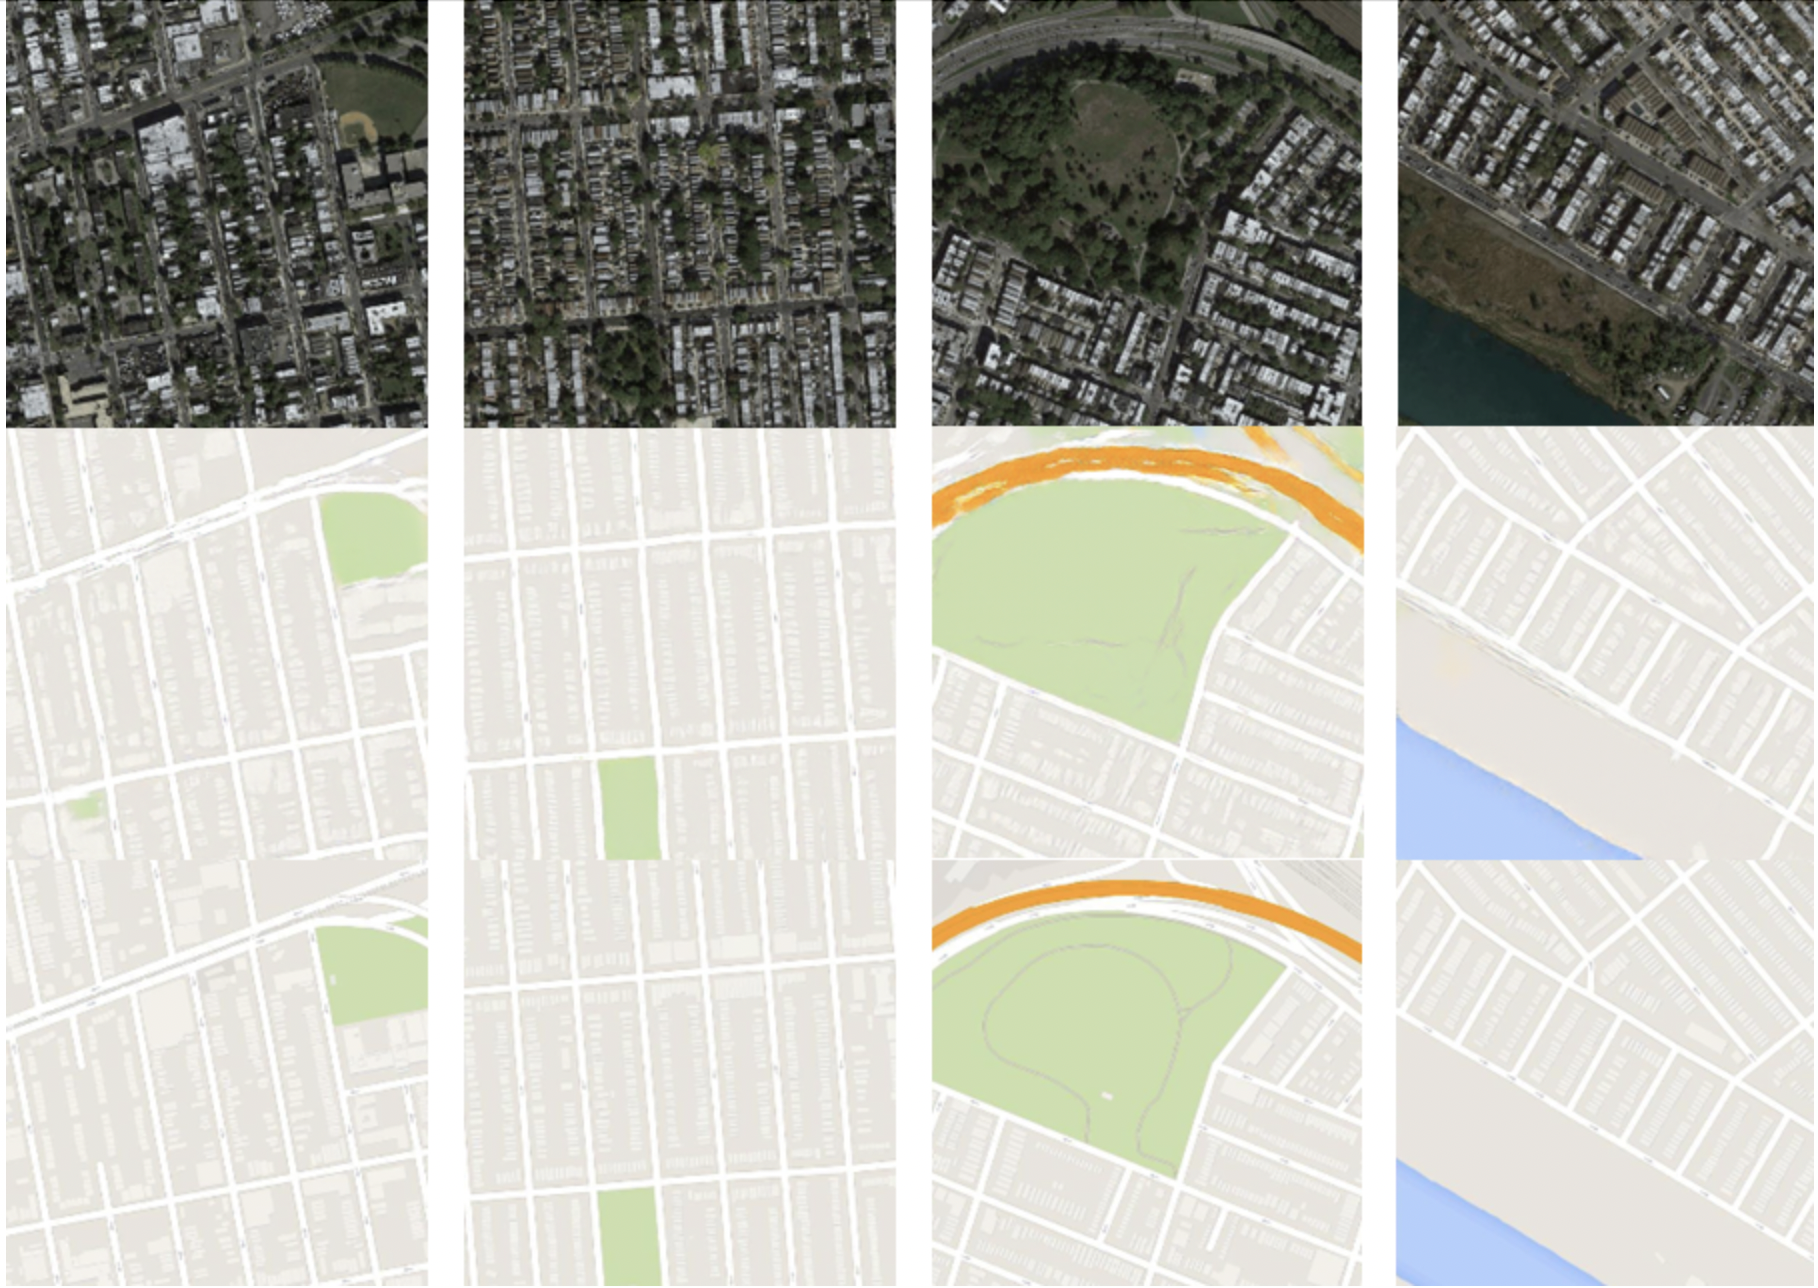
\includegraphics[width=\linewidth,height=7cm]{figures/2.png}
    \caption{ Satellite To Map Image Conversion }
    \label{fig:GAN model}
\end{figure}



\subsection{GAN Model}
	
\par	GANs, or Generative Adversarial Networks, are a type of generative modelling that employs deep learning techniques such as convolutional neural networks. In machine learning, generative modelling is an unsupervised learning job that entails automatically detecting and learning regularities or patterns in input data so that the model may be used to produce or output new examples that could have been drawn from the original dataset. GANs are a clever way of training a generative model by framing the problem as a supervised learning problem with two sub-models: the generator model, which we train to generate new examples, and the discriminator model, which tries to classify examples as real (from the domain) or fake (from outside the domain) (generated). Both models have undergone training.

	
	\begin{figure}[h!]
    \centering
    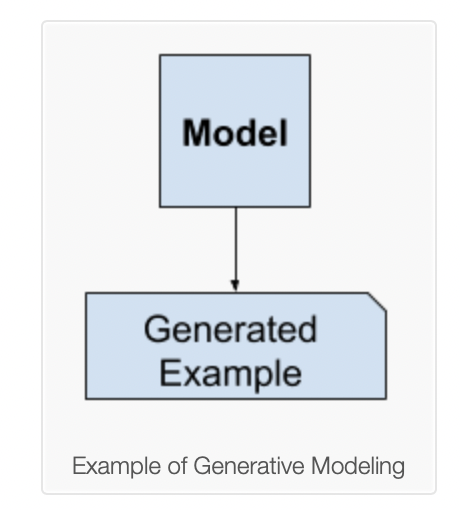
\includegraphics[width=\linewidth,height=7cm]{figures/3.png}
    \caption{ Example of generative modeling}
    \label{fig:GAN model}
\end{figure}



	\begin{figure}[h!]
    \centering
    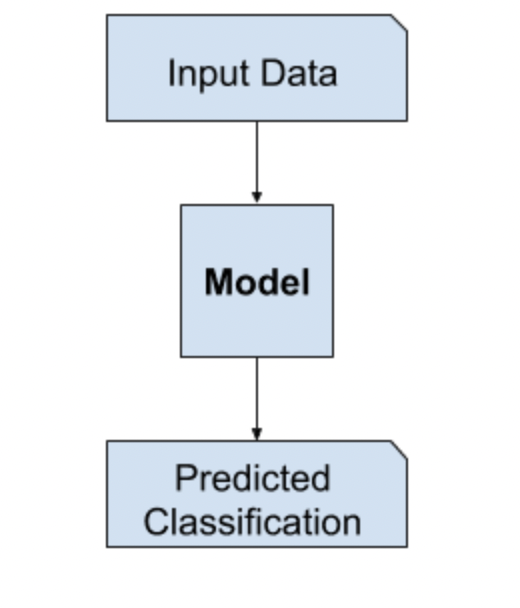
\includegraphics[width=\linewidth,height=7cm]{figures/4.png}
    \caption{  Example of discriminate modeling}
    \label{fig:GAN model}
\end{figure}


	\begin{figure}[h!]
    \centering
    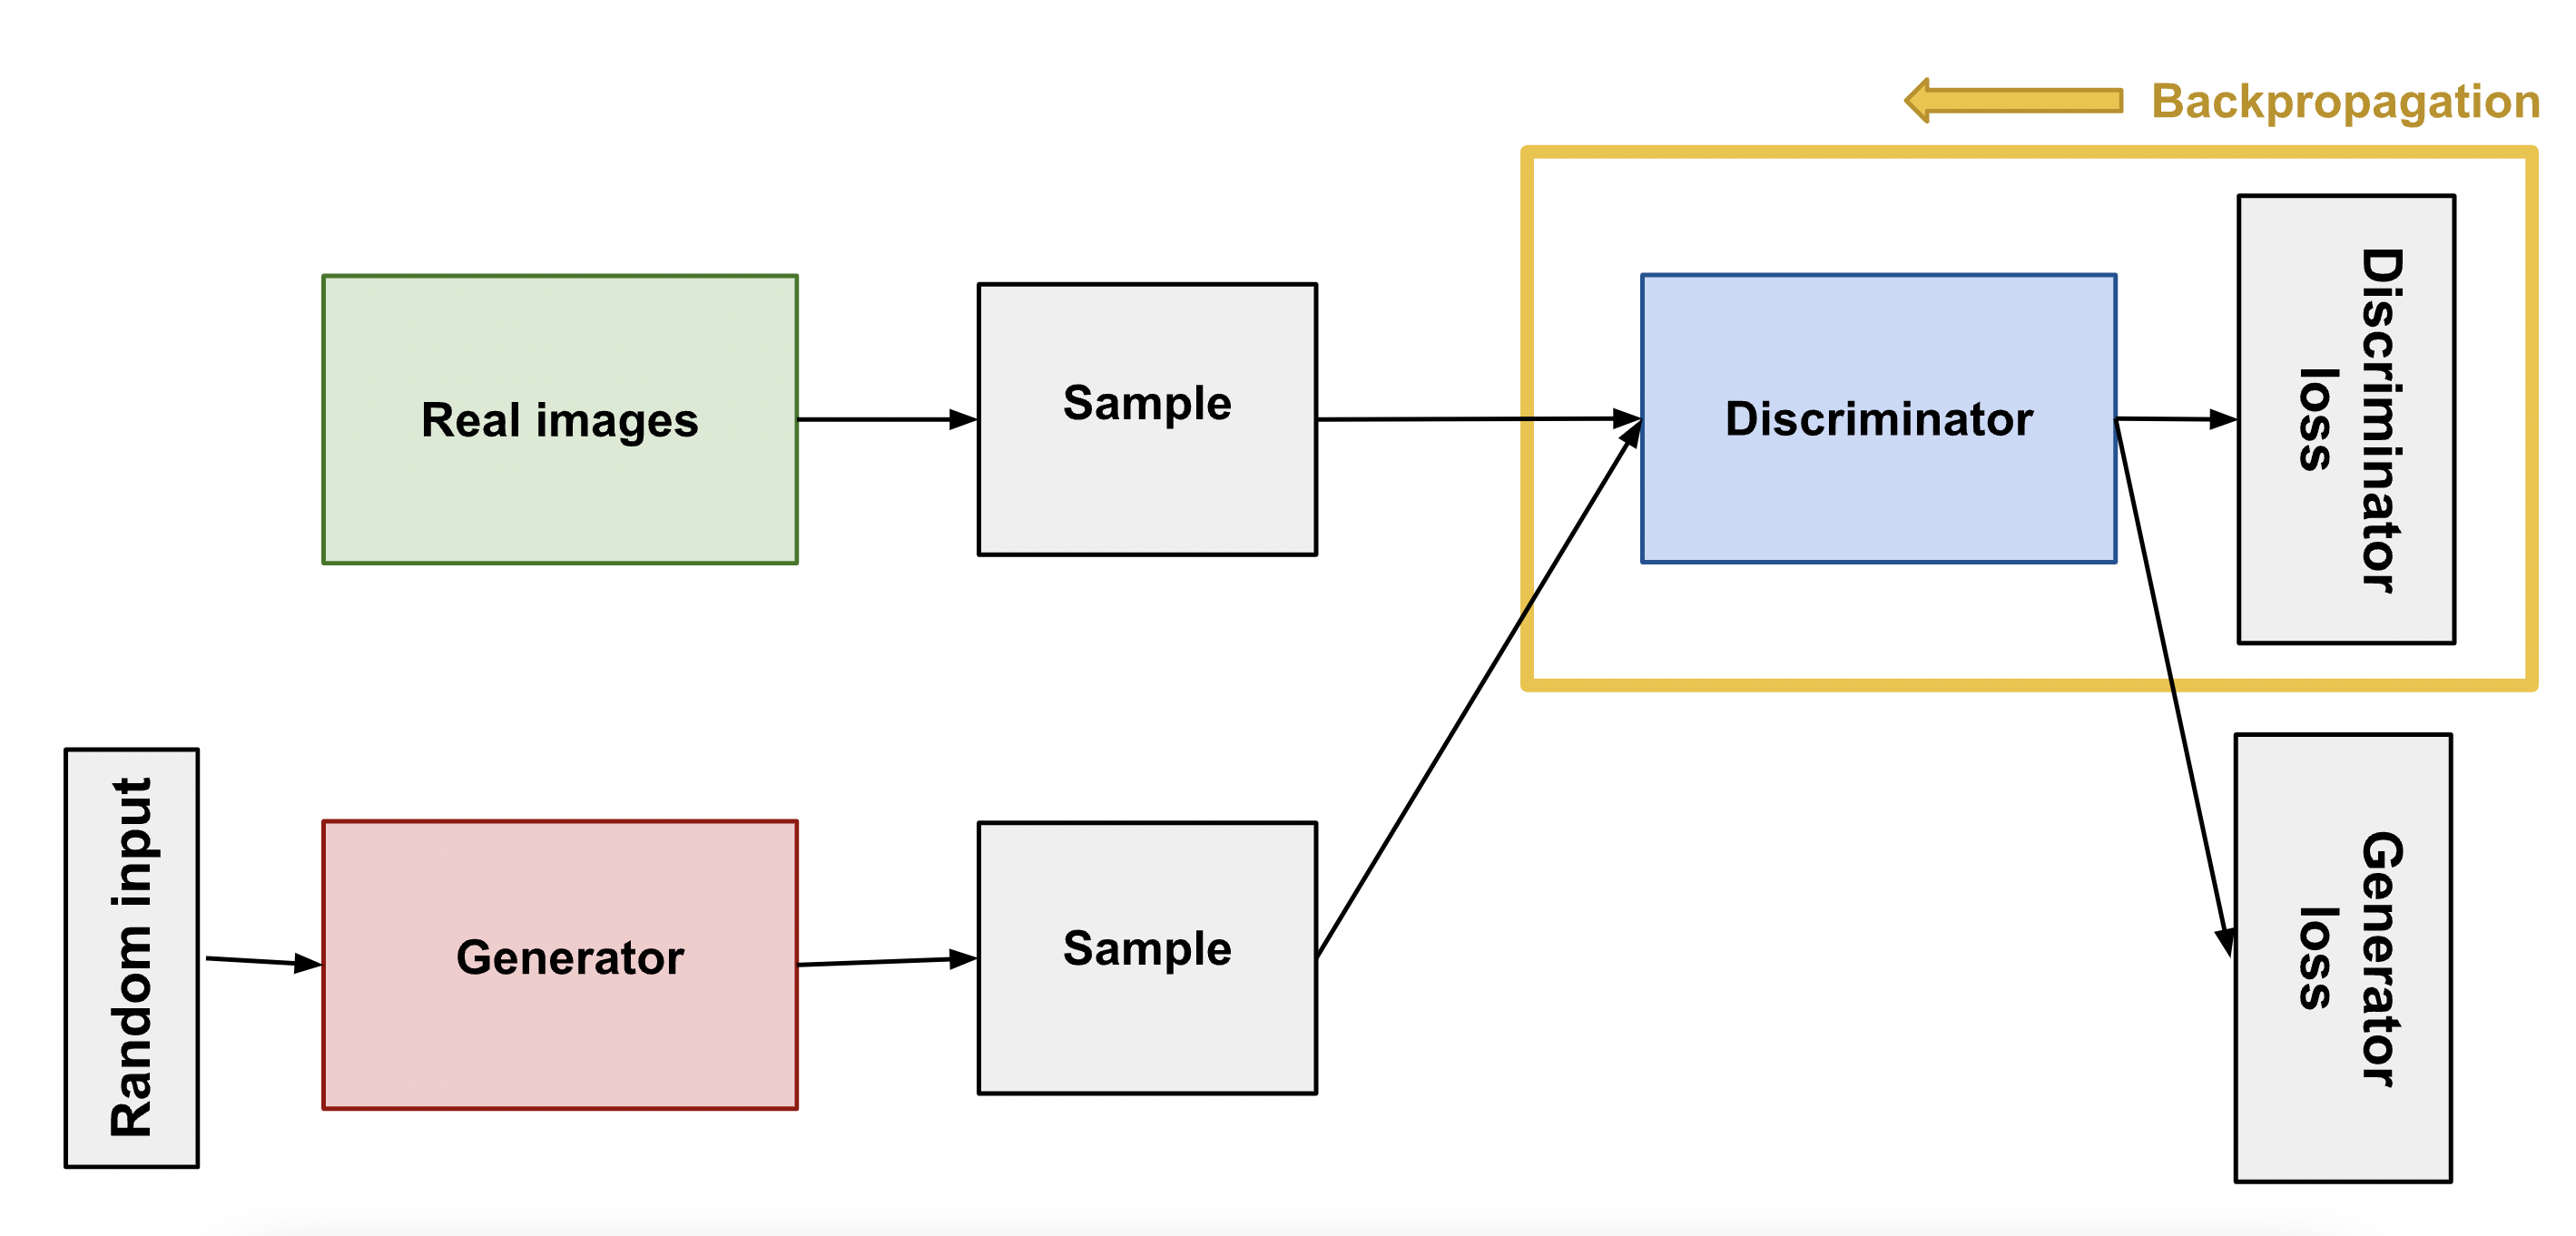
\includegraphics[width=\linewidth,height=7cm]{figures/1.png}
    \caption{ Architecture of GAN model}
    \label{fig:GAN model}
\end{figure}



\par  